
\documentclass[letterpaper,hide notes,xcolor={table,svgnames},pdftex,10pt]{beamer}
\def\showexamples{t}


%\usepackage[svgnames]{xcolor}

%% Demo talk
%\documentclass[letterpaper,notes=show]{beamer}

\usecolortheme{crane}
\setbeamertemplate{navigation symbols}{}

\usetheme{MyPittsburgh}
%\usetheme{Frankfurt}

%\usepackage{tipa}

\usepackage{hyperref}
\usepackage{graphicx,xspace}
\usepackage[normalem]{ulem}
\usepackage{multicol}

\newcommand\SF[1]{$\bigstar$\footnote{SF: #1}}

\usepackage[default]{sourcesanspro}
\usepackage[T1]{fontenc}

\newcounter{tmpnumSlide}
\newcounter{tmpnumNote}

% old question code
%\newcommand\question[1]{{$\bigstar$ \small \onlySlide{2}{#1}}}
% \newcommand\nquestion[1]{\ifdefined \presentationonly \textcircled{?} \fi \note{\par{\Large \textbf{?}} #1}}
% \newcommand\nanswer[1]{\note{\par{\Large \textbf{A}} #1}}


 \newcommand\mnote[1]{%
   \addtocounter{tmpnumSlide}{1}
   \ifdefined\showcues {~\tiny\fbox{\arabic{tmpnumSlide}}}\fi
   \note{\setlength{\parskip}{1ex}\addtocounter{tmpnumNote}{1}\textbf{\Large \arabic{tmpnumNote}:} {#1\par}}}

\newcommand\mmnote[1]{\note{\setlength{\parskip}{1ex}#1\par}}

%\newcommand\mnote[2][]{\ifdefined\handoutwithnotes {~\tiny\fbox{#1}}\fi
% \note{\setlength{\parskip}{1ex}\textbf{\Large #1:} #2\par}}

%\newcommand\mnote[2][]{{\tiny\fbox{#1}} \note{\setlength{\parskip}{1ex}\textbf{\Large #1:} #2\par}}

\newcommand\mquestion[2]{{~\color{red}\fbox{?}}\note{\setlength{\parskip}{1ex}\par{\Large \textbf{?}} #1} \note{\setlength{\parskip}{1ex}\par{\Large \textbf{A}} #2\par}\ifdefined \presentationonly \pause \fi}

\newcommand\blackboard[1]{%
\ifdefined   \showblackboard
  {#1}
  \else {\begin{center} \fbox{\colorbox{blue!30}{%
         \begin{minipage}{.95\linewidth}%
           \hspace{\stretch{1}} Some space intentionally left blank; done at the blackboard.%
         \end{minipage}}}\end{center}}%
         \fi%
}



%\newcommand\q{\tikz \node[thick,color=black,shape=circle]{?};}
%\newcommand\q{\ifdefined \presentationonly \textcircled{?} \fi}

\usepackage{listings}
\lstset{%
  keywordstyle=\bfseries,
  aboveskip=15pt,
  belowskip=15pt,
  captionpos=b,
  identifierstyle=\ttfamily,
  escapeinside={(*@}{@*)},
  stringstyle=\ttfamiliy,
  frame=lines,
  numbers=left, basicstyle=\scriptsize, numberstyle=\tiny, stepnumber=0, numbersep=2pt}

\usepackage{siunitx}
\newcommand\sius[1]{\num[group-separator = {,}]{#1}\si{\micro\second}}
\newcommand\sims[1]{\num[group-separator = {,}]{#1}\si{\milli\second}}
\newcommand\sins[1]{\num[group-separator = {,}]{#1}\si{\nano\second}}
\sisetup{group-separator = {,}, group-digits = true}

%% -------------------- tikz --------------------
\usepackage{tikz}
\usetikzlibrary{positioning}
\usetikzlibrary{arrows,backgrounds,automata,decorations.shapes,decorations.pathmorphing,decorations.markings,decorations.text}

\tikzstyle{place}=[circle,draw=blue!50,fill=blue!20,thick, inner sep=0pt,minimum size=6mm]
\tikzstyle{transition}=[rectangle,draw=black!50,fill=black!20,thick, inner sep=0pt,minimum size=4mm]

\tikzstyle{block}=[rectangle,draw=black, thick, inner sep=5pt]
\tikzstyle{bullet}=[circle,draw=black, fill=black, thin, inner sep=2pt]

\tikzstyle{pre}=[<-,shorten <=1pt,>=stealth',semithick]
\tikzstyle{post}=[->,shorten >=1pt,>=stealth',semithick]
\tikzstyle{bi}=[<->,shorten >=1pt,shorten <=1pt, >=stealth',semithick]

\tikzstyle{mut}=[-,>=stealth',semithick]

\tikzstyle{treereset}=[dashed,->, shorten >=1pt,>=stealth',thin]

\usepackage{ifmtarg}
\usepackage{xifthen}
\makeatletter
% new counter to now which frame it is within the sequence
\newcounter{multiframecounter}
% initialize buffer for previously used frame title
\gdef\lastframetitle{\textit{undefined}}
% new environment for a multi-frame
\newenvironment{multiframe}[1][]{%
\ifthenelse{\isempty{#1}}{%
% if no frame title was set via optional parameter,
% only increase sequence counter by 1
\addtocounter{multiframecounter}{1}%
}{%
% new frame title has been provided, thus
% reset sequence counter to 1 and buffer frame title for later use
\setcounter{multiframecounter}{1}%
\gdef\lastframetitle{#1}%
}%
% start conventional frame environment and
% automatically set frame title followed by sequence counter
\begin{frame}%
\frametitle{\lastframetitle~{\normalfont(\arabic{multiframecounter})}}%
}{%
\end{frame}%
}
\makeatother

\makeatletter
\newdimen\tu@tmpa%
\newdimen\ydiffl%
\newdimen\xdiffl%
\newcommand\ydiff[2]{%
    \coordinate (tmpnamea) at (#1);%
    \coordinate (tmpnameb) at (#2);%
    \pgfextracty{\tu@tmpa}{\pgfpointanchor{tmpnamea}{center}}%
    \pgfextracty{\ydiffl}{\pgfpointanchor{tmpnameb}{center}}%
    \advance\ydiffl by -\tu@tmpa%
}
\newcommand\xdiff[2]{%
    \coordinate (tmpnamea) at (#1);%
    \coordinate (tmpnameb) at (#2);%
    \pgfextractx{\tu@tmpa}{\pgfpointanchor{tmpnamea}{center}}%
    \pgfextractx{\xdiffl}{\pgfpointanchor{tmpnameb}{center}}%
    \advance\xdiffl by -\tu@tmpa%
}
\makeatother
\newcommand{\copyrightbox}[3][r]{%
\begin{tikzpicture}%
\node[inner sep=0pt,minimum size=2em](ciimage){#2};
\usefont{OT1}{phv}{n}{n}\fontsize{4}{4}\selectfont
\ydiff{ciimage.south}{ciimage.north}
\xdiff{ciimage.west}{ciimage.east}
\ifthenelse{\equal{#1}{r}}{%
\node[inner sep=0pt,right=1ex of ciimage.south east,anchor=north west,rotate=90]%
{\raggedleft\color{black!50}\parbox{\the\ydiffl}{\raggedright{}#3}};%
}{%
\ifthenelse{\equal{#1}{l}}{%
\node[inner sep=0pt,right=1ex of ciimage.south west,anchor=south west,rotate=90]%
{\raggedleft\color{black!50}\parbox{\the\ydiffl}{\raggedright{}#3}};%
}{%
\node[inner sep=0pt,below=1ex of ciimage.south west,anchor=north west]%
{\raggedleft\color{black!50}\parbox{\the\xdiffl}{\raggedright{}#3}};%
}
}
\end{tikzpicture}
}


%% --------------------

%\usepackage[excludeor]{everyhook}
%\PushPreHook{par}{\setbox0=\lastbox\llap{MUH}}\box0}

%\vspace*{\stretch{1}

%\setbox0=\lastbox \llap{\textbullet\enskip}\box0}

\setlength{\parskip}{\fill}

\newcommand\noskips{\setlength{\parskip}{1ex}}
\newcommand\doskips{\setlength{\parskip}{\fill}}

\newcommand\xx{\par\vspace*{\stretch{1}}\par}
\newcommand\xxs{\par\vspace*{2ex}\par}
\newcommand\tuple[1]{\langle #1 \rangle}
\newcommand\code[1]{{\sf \footnotesize #1}}
\newcommand\ex[1]{\uline{Example:} \ifdefined \presentationonly \pause \fi
  \ifdefined\showexamples#1\xspace\else{\uline{\hspace*{2cm}}}\fi}

\newcommand\ceil[1]{\lceil #1 \rceil}


\AtBeginSection[]
{
   \begin{frame}
       \frametitle{Outline}
       \tableofcontents[currentsection]
   \end{frame}
}



\pgfdeclarelayer{edgelayer}
\pgfdeclarelayer{nodelayer}
\pgfsetlayers{edgelayer,nodelayer,main}

\tikzstyle{none}=[inner sep=0pt]
\tikzstyle{rn}=[circle,fill=Red,draw=Black,line width=0.8 pt]
\tikzstyle{gn}=[circle,fill=Lime,draw=Black,line width=0.8 pt]
\tikzstyle{yn}=[circle,fill=Yellow,draw=Black,line width=0.8 pt]
\tikzstyle{empty}=[circle,fill=White,draw=Black]
\tikzstyle{bw} = [rectangle, draw, fill=blue!20, 
    text width=4em, text centered, rounded corners, minimum height=2em]
    
    \newcommand{\CcNote}[1]{% longname
	This work is licensed under the \textit{Creative Commons #1 3.0 License}.%
}
\newcommand{\CcImageBy}[1]{%
	\includegraphics[scale=#1]{creative_commons/cc_by_30.pdf}%
}
\newcommand{\CcImageSa}[1]{%
	\includegraphics[scale=#1]{creative_commons/cc_sa_30.pdf}%
}
\newcommand{\CcImageNc}[1]{%
	\includegraphics[scale=#1]{creative_commons/cc_nc_30.pdf}%
}
\newcommand{\CcGroupBySa}[2]{% zoom, gap
	\CcImageBy{#1}\hspace*{#2}\CcImageNc{#1}\hspace*{#2}\CcImageSa{#1}%
}
\newcommand{\CcLongnameByNcSa}{Attribution-NonCommercial-ShareAlike}

\newenvironment{changemargin}[1]{% 
  \begin{list}{}{% 
    \setlength{\topsep}{0pt}% 
    \setlength{\leftmargin}{#1}% 
    \setlength{\rightmargin}{1em}
    \setlength{\listparindent}{\parindent}% 
    \setlength{\itemindent}{\parindent}% 
    \setlength{\parsep}{\parskip}% 
  }% 
  \item[]}{\end{list}} 




\title{Lecture 30 --- Ethics: Introduction }

\author{Jeff Zarnett \\ \small \texttt{jzarnett@uwaterloo.ca}}
\institute{Department of Electrical and Computer Engineering \\
  University of Waterloo}
\date{\today}


\begin{document}

\begin{frame}
  \titlepage

\begin{center}
  \small{Acknowledgments: Douglas Harder~\cite{dwh}, Julie Vale~\cite{jv}}
  \end{center}
\end{frame}



\begin{frame}
\frametitle{The Runaway Train Car}

Ethics are about moral principles; about how we know what is ``right'' and what is ``wrong''. 

Instead of starting with a long discussion of the subject, let's do an exercise where we look at some ethical situations. 

In all of them, we have to make a decision.

\end{frame}



\begin{frame}
\frametitle{The Runaway Train Car, Scenario 1}


In the first example, our decision is binary:\\

\begin{enumerate}[A.]
	\item Do nothing.
	\item Pull the lever.
\end{enumerate}

\begin{center}
	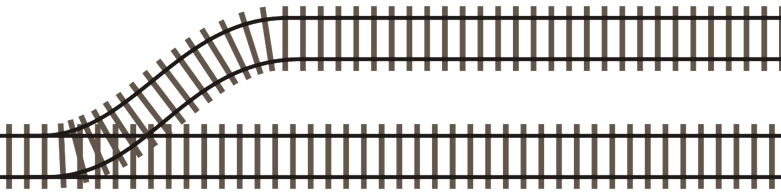
\includegraphics[width=\textwidth]{images/crazytrain}
\end{center}


1A: There are five workers on the current line and one on the parallel track.\\
\quad What do you do?

\end{frame}

\begin{frame}
\frametitle{The Runaway Train Car, Scenario 1}

1B. What if there are only two workers on the main line?

1C. What if there are 50 workers on the main line?

1D: What if there are 20 on the main and 4 on the side?

1E: What if there is a car with an infant on the side line?

\end{frame}



\begin{frame}
\frametitle{The Runaway Train Car, Scenario 1}

Suppose the train car is moving very fast and there is an 80\% chance that the deflection onto the side line will cause the train car to derail, killing no one.

1F: What if there are five workers on the main line and one on the side?

1G: What if there are five workers on each track?


\end{frame}


\begin{frame}
\frametitle{The Runaway Train Car, Scenario 2}

In the next example, our decision is still binary:\\

\begin{enumerate}[A.]
	\item Do nothing.
	\item Push.
\end{enumerate}

A train is speeding down the tracks, but you are standing on an overpass. There is a very fat man on the overpass next to you. 

2A: There are five workers up ahead. If you push the fat person over, the train will hit him and derail and the workers will be saved. What do you do?


\end{frame}

\begin{frame}
\frametitle{The Runaway Train Car, Scenario 2}

2B: What if there are 50 workers?

2C: What if the railway car is packed with explosives and it's headed straight for Parliament\footnote{Remember, remember the fifth of November...}?

2D: What if the fat man asks you to help him over the railing?

Is this even a question of ethics if you choose to jump yourself (i.e., you are the fat person in this scenario)?


\end{frame}



\begin{frame}
\frametitle{Car Crash}

A family of six is involved in an motor vehicle collision. 

Five are severely injured; one is critically injured.

All are brought to the hospital. 

Without immediate attention the five may very well die; the sixth, however, is dying most acutely.

\end{frame}



\begin{frame}
\frametitle{Car Crash}

Is it ethical to sacrifice the critically injured family member to save the others?  

(Assume all are unconscious.)

\end{frame}

\begin{frame}
\frametitle{Car Crash}

Suppose instead there are five seriously injured individuals in an accident, all requiring immediate attention.

In the waiting room is a patient who is coming to see the result of his blood test --looking over the charts, you notice that he is a perfect match for all the five injured.

Do you sacrifice that individual to save the five?  

\end{frame}



\begin{frame}
\frametitle{Professional Engineering Ethics}

The definition of professional misconduct includes those behaviours that a professional engineer in Ontario must not engage in.

These define an absolute line which must not be crossed.

Note that one can be guilty of professional misconduct even if there are no negative consequences.

In general, however, complaints are a result of an action or behaviour having a negative consequence.


\end{frame}



\begin{frame}
\frametitle{Professional Engineering Ethics}

\begin{itemize}
	\item Should we regulate how professional engineers interact with other professionals?
	\item Should professional engineers exaggerate their abilities or the abilities of the profession?
	\item Should professional engineers malign the character of others in the profession?
	\item You find that your designs had a flaw due to an unknown effect not anticipated in normal engineering practice:  is it sufficient to fix the mistake but not tell anyone about it?
	\item Is it right to take credit for the work done by your subordinates and co-op students working under you?
\end{itemize}

\end{frame}



\begin{frame}
\frametitle{Morals}

A moral, meaning a custom or a habit is an action, behaviour, character trait or desire that has been determined to be:

\begin{itemize}
	\item Right or wrong
	\item Good or bad
	\item Saintly or evil
	\item Honourable or dishonourable
	\item Brave or cowardly
\end{itemize}

It is based on a general consensus of society. They are not based in law or regulations;
there are immoral rules and immoral orders.


\end{frame}



\begin{frame}
\frametitle{Ethics}

The study of ethics or moral philosophy is the study of human interactions.

It is for determining or recommending whether an actions, behaviours, conduct or desires is right or wrong, including:

\begin{itemize}
	\item Actions
	\item Behaviours
	\item Characteristics
	\item Desires
\end{itemize}


\end{frame}



\begin{frame}
\frametitle{Ethics}

There are two general definitions of ethics.

1. A collection or system of moral principles or rules of conduct by which a person or association is guided.


2. The science of morals; the department of study concerned with the principles of human duty.

\end{frame}



\begin{frame}
\frametitle{Hippocratic Oath}

The Hippocratic Oath and Professional Engineers Ontario Code of Ethics are two examples of collections of rules of conduct.

In many jurisdictions, a code of ethics defines the boundary between professional conduct and misconduct.

We will see later, that PEO's Code of Ethics provide a guide to conduct while, as we've seen, misconduct is explicitly defined in the regulations.

\end{frame}



\begin{frame}
\frametitle{Ethics: The Science of Morals}


Ethics is itself broken into numerous categories:
\begin{itemize}
	\item \textbf{Meta-ethics}:
the theoretical inquiry of moral principles and how their truth values (if any) may be determined
	\item \textbf{Normative ethics}:
Concerning the practical means of determining a moral course of action
	\item \textbf{Applied ethics}:
Situation-based moral outcomes
	\item \textbf{Descriptive Ethics}:
The study of extant ethical behaviour and comparative analysis
	\item \textbf{Moral psychology}:
The scientific study of the development and evolution of ethical behaviour
\end{itemize}

\end{frame}



\begin{frame}
\frametitle{Normative Ethics}

We will focus entirely on normative ethics:

\begin{itemize}
\item Concerning the practical means of determining a moral course of action
\item Normative ethics tends to be prescriptive:  it prescribes how to deal with a particular ethical situation
\item Descriptive ethics is empirical:  it investigates a society's response in dealing with a particular ethical situation
\end{itemize}

\end{frame}



\begin{frame}
\frametitle{Virtue Ethics}

Virtue ethics asks how a response to a situation will affect the perceived character of the person.

Helping a person in need would be charitable, and viewed positively.

A decision on whether or not to lie would be judged on how that falsehood reflects on the individual's character.

First discussed in western philosophy by Plato and then Aristotle.

Plato lists four cardinal moral virtues: courage, temperance, justice, prudence.

Each is the golden mean between two extremes
\end{frame}



\begin{frame}
\frametitle{Role Ethics}

Morality is derived from people's relationship with their community and is not individualistic.

Confuianism demonstrates this through
the concept of filial piety as a desire and
not only as an action

\begin{quote}
In serving his parents,\\
a filial son reveres them in daily life;\\
he makes them happy while he nourishes them;\\
he takes anxious care of them in sickness;\\
he shows great sorrow over their death; and\\
he sacrifices to them with solemnity.\\
\end{quote}


\end{frame}


\begin{frame}
\frametitle{References \& Disclaimer}
\bibliographystyle{alphaurl}
\setbeamertemplate{bibliography item}{\insertbiblabel}
{\scriptsize
\bibliography{290}
}
\vfill

{\tiny Disclaimer: the material presented in these lectures slides is intended for use in the course ECE~290 at the University of Waterloo and should not be relied upon as legal advice. Any reliance on these course slides by any party for any other purpose are the responsibility of such parties.  The author(s) accept(s) no responsibility for damages, if any, suffered by any party as a result of decisions made or actions based on these course slides for any other purpose than that for which it was intended.\par}


\end{frame}


\end{document}

